\subsection{Вырожденные звёзды}
\term{Вырожденные звезды}~--- звезды, в которых силам гравитации противостоят силы давление вырожденного газа. К таким относятся \imp{белые карлики} и \imp{нейтронные звезды}.

\begin{wrapfigure}[16]{r}{0.4\tw}
    \centering
    \vspace{-0.7pc}
    \tikzsetnextfilename{mass-radius-wd}
    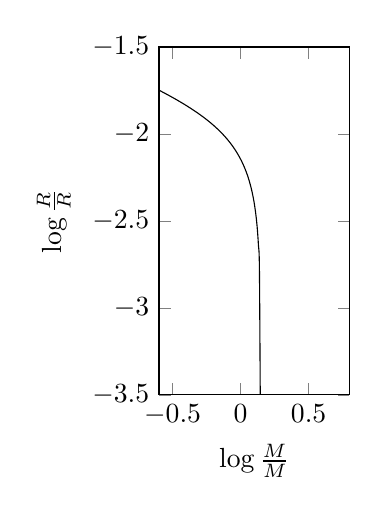
\begin{tikzpicture}
        \begin{axis}[
            width    =    4cm,
            height    =    6cm,
            xmax     =    0.8,
            xmin    =    -0.6,
            ymax    =    -1.5,
            ymin     =     -3.5,
            ylabel    =    {$\log\frac{R}{R_{\astrosun}}$},
            xlabel     =     {$\log\frac{M}{M_{\astrosun}}$}
        ]
            \addplot [domain=-0.6:0.146, samples = 100, black, smooth]{
            ln(
                (
                    (1.4 / (10^x))^0.66 
                    - 
                    ((10^x) / 1.4)^0.66
                )^0.5 
                / 93.5
            ) / ln(10)};
        \end{axis}
    \end{tikzpicture}
    \caption{Зависимость масса-радиус для белых карликов}
    \label{pic:mass-radius-wd}
\end{wrapfigure}

\term{Белые карлики}~--- проэволюционировавшие звёзды лишённые собственных источников термоядерной энергии и светящие за счёт остывания. Масса белого карлика находится в диапазоне от $0.6M_{\odot}$ до $1.44 M_{\odot}$. Верхняя границы массы белого карлика называется пределом Чандрасекара, звезда с массой больше данного предела не может существовать как белый карлик. Радиус белых карликов примерно в $10^2$ раз меньше солнечного, т.е. можно считать, что $R_\text{БК} \simeq R_\oplus$. Плотность белых карликов лежит в диапазоне $10^7$\,--\,$10^{10}$~$\text{кг}/\text{м}^3$. Зависимость масса-радиус для белых карликов имеет сложную форму \lookPicRef{pic:mass-radius-wd}. Вертикальная асимптота на графике соотвтетствует пределу Чандрасекара. 

Спектры белых карликов отличаются от спектров невырожденных звёзд. Главной особенностью являются \imp{широкие линии поглощения}, также примечательно малое присутствие или вовсе отсутсвие слабых линий в спектре. Белые карлики принято выделять в отдельный спектральный класс D, а подклассы выделяют по принципу присутствия тех или иных спектральных линий в спектре. Основные подклассы: \term{DA} и \term{DB}. Остальные подклассы представляются немногочисленными. Между этими двумя подклассами наблюдается количественное соотношение 80:20, оно объясняется эволюцией: на последних стадиях жизни у пульсирующий красных гигантов уже присутствует вырожденное ядро окруженное водородным слоевым источником. Вследствие накопления гелия в ядре периодически происходит \imp{гелиевая вспышка} — вырождение внешних гелиевых слоёв ядра и резкое ускорение реакций. Однако после выгорания накопленного гелия происходит очередной поджог водородного слоевого источника. Красный гигант может сбросить оболочку в любой стадии, при сбросе в период гелиевой вспышки образуется гелиевый белый карлик класса DB, а если сброс произошел в период горения водородного слоевого источника — обнажится водородный белый карлик класса DA. Длительность гелиевой вспышки составляет около 20\% от длительности цикла пульсации, что и объясняет соотношение водородных и гелиевых карликов. На \picRef{pic:mass-radius-wd} приведены типовые спектры белых карликов класса DA и класса DB.


\begin{figure}[h!]
    \centering
    \tikzsetnextfilename{spectrum-wd}
    \begin{tikzpicture}
        \begin{groupplot}[
            group style={
            	group name=wdplot,
                group size=1 by 2,
                vertical sep=0.5cm
            },
            width=\tw,
            height=5cm
            ]
            \nextgroupplot[
                yticklabels={0, 1},
                xticklabels={},
                xmin=3800, xmax=6200,
                ytick={0, 1},
                xtick={4000, 4500, 5000, 5500, 6000},
            ]
            \addplot[black, smooth] table[col sep=comma, x=wavelength, y=flux] {data/spectrum-DA.csv};
            
            \nextgroupplot[
                yticklabels={0, 1},
                xmin=3800, xmax=6200,
                ytick={0, 1},
                xtick={4000, 4500, 5000, 5500, 6000},
                xlabel={Длина волны $\lambda,~\,\mathring{\text{A}}$}
            ]
            \addplot[black, smooth] table[col sep=comma, x=wavelength, y=flux] {data/spectrum-DB.csv};
        \end{groupplot}
        \path (wdplot c1r1.outer north west)
          -- node[anchor=south,rotate=90] {\textsf{Относительная интенсивность}}
          (wdplot c1r2.outer south west)
    	;
    \end{tikzpicture}
    \caption{Спектр водородного и гелиевого белых карликов}
    \label{pic:spectrum-wd}
\end{figure}

\term{Нейтронная звезда}~--- сверхплотная звезда, образующаяся в результате взрыва Сверхновой. Вещество нейтронной звезды состоит в основном из нейтронов. Масса нейтронной звезды лежит в пределах от $0.1M_{\odot}$ до $2$\,--\,$2.8M_{\odot}$ (предел Оппенгеймера-Волкова). Размер данной звезды составляет лишь $10$\,--\,$20$~км, а плотность составляет $10^{16}$\,--\,$10^{18}$ $\text{кг}/\text{м}^3$.  Дальнейшему гравитационному сжатию нейтронной звезды препятствует давление ядерной материи, возникающее за счёт взаимодействия нейтронов. Так как нейтронные звёзды образуются в результате  коллапса массивных звёзд, то из-за сохранения момента импульса скорость их вращения может достигать $10^5$~км/с. При наличии сильного магнитного поля и быстром вращении нейтронная звзеда может наблюдаться с Земли как \term{пульсар}.


